\chapter{Teoría de grafos}
    Con el propósito de abordar el estudio de las redes de transporte público sobre bases conceptuales sólidas, en este capítulo presentamos las definiciones y herramientas fundamentales de la teoría de grafos. Nos interesa precisar, en particular, la noción de \emph{camino} y su papel en la representación de trayectorias en una red; asimismo, discutimos medidas de \emph{centralidad} que permiten evaluar la relevancia relativa de los vértices dentro de la estructura global. Finalmente, revisamos algoritmos clásicos para el cálculo de caminos óptimos entre pares de vértices.

    \subsection{Fundamentos de la teoría de grafos}

    Los problemas de movilidad urbana requieren modelos que abstraigan la complejidad de la ciudad sin perder los elementos esenciales de conectividad. La \emph{teoría de grafos} provee ese andamiaje formal: reduce las interacciones físicas a vértices y aristas y, a partir de allí, permite
    cuantificar eficiencia, robustez y vulnerabilidad de la red (Rodrigues, 2013).

    \subsection{Definiciones y notación}
    A efectos terminológicos, adoptamos la siguiente convención: emplearemos el término \emph{vértice} y, cuando corresponda al lenguaje aplicado de redes, \emph{nodo} como sinónimo. En lo sucesivo, preferiremos “vértice” para mantener la consistencia formal. Llamaremos \emph{arista} (o \emph{enlace}) a cada conexión entre vértices.

    \begin{definition}
    Un \textbf{grafo} $G$ es un par ordenado
    \begin{equation}
        G = (V,E),
    \end{equation}
    donde $V$ es un conjunto no vacío de \emph{vértices} (también denominados \emph{nodos}) y $E \subseteq V\times V$ es el conjunto de \emph{aristas}. (Rodrigues, 2013).
    \end{definition}

    Salvo indicación en contrario, trabajaremos con \emph{dígrafos} (grafos dirigidos) ponderados y supondremos que no existen bucles, esto es, $(v,v) \notin E$ para todo $v\in V$.

    \subsubsection{Tipos de grafos}
        Dependiendo de las propiedades de $E$, los grafos pueden clasificarse en diversas categorías:

        \begin{itemize}
            \item \textbf{Grafo no dirigido}: las aristas no tienen orientación; en particular, $(u, v) \in E$ implica $(v, u) \in E$.

                \begin{center}
                    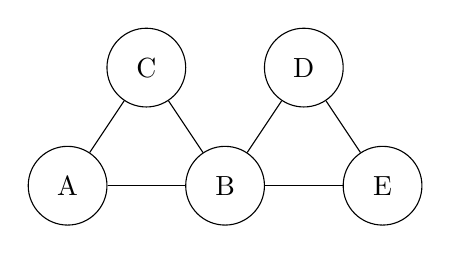
\begin{tikzpicture}[scale=1, every node/.style={draw, circle, minimum size=1cm}]
                        \node (A) at (0,0) {A};
                        \node (B) at (2,0) {B};
                        \node (C) at (1,1.5) {C};
                        \node (D) at (3,1.5) {D};
                        \node (E) at (4,0) {E};

                        \draw (A) -- (B);
                        \draw (A) -- (C);
                        \draw (B) -- (C);
                        \draw (B) -- (D);
                        \draw (B) -- (E);
                        \draw (D) -- (E);
                    \end{tikzpicture}
                \end{center}

            \item \textbf{Grafo dirigido (dígrafo)}: cada arista posee una orientación; por tanto, $(u, v) \in E$ no implica necesariamente $(v, u) \in E$. En tal caso, diremos que existe una arista dirigida de $u$ hacia $v$.

                \begin{center}
                    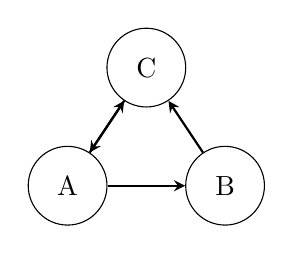
\begin{tikzpicture}[scale=1, every node/.style={draw, circle, minimum size=1cm}, >=stealth]
                        \node (A) at (0,0) {A};
                        \node (B) at (2,0) {B};
                        \node (C) at (1,1.5) {C};

                        \draw[->, thick] (A) -- (B);
                        \draw[->, thick] (B) -- (C);
                        \draw[->, thick] (C) -- (A);
                        \draw[->, thick] (A) -- (C);
                    \end{tikzpicture}
                \end{center}
            \item \textbf{Grafo ponderado}: a cada arista $(u, v) \in E$ se le asigna un peso $w(u, v) \in \mathbb{R}$ que puede representar costos, distancias u otras métricas relevantes. Un grafo puede ser simultáneamente ponderado y dirigido (o no dirigido).
                \begin{center}
                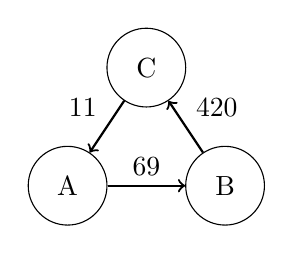
\begin{tikzpicture}[scale=1,
                    vertex/.style={draw, circle, minimum size=1cm}
                    ]
                    % Definición de vértices
                    \node[vertex] (A) at (0,0) {A};
                    \node[vertex] (B) at (2,0) {B};
                    \node[vertex] (C) at (1,1.5) {C};

                    % Aristas con etiquetas; se anula el estilo global para estos nodos
                    \draw[->, thick] (A) -- node[above, draw=none, fill=none] {69} (B);
                    \draw[->, thick] (B) -- node[above right, draw=none, fill=none] {420} (C);
                    \draw[->, thick] (C) -- node[above left, draw=none, fill=none] {11} (A);
                \end{tikzpicture}
            \end{center}

        \end{itemize}

    \subsection{Propiedades fundamentales de los grafos}
        Los grafos poseen propiedades matemáticas que permiten su análisis estructural.
        Para este estudio resultan especialmente útiles la \textit{conectividad}, que posibilita cuantificar la relevancia de un vértice con respecto a los demás, y los \textit{caminos}, que representan trayectorias, entre otros conceptos.

        \subsubsection{Subgrafos}

        Un subgrafo $H = (V_H, E_H)$ de un grafo $G = (V, E)$ es un grafo tal que $V_H \subseteq V$ y $E_H \subseteq E$.
        Es decir, un subgrafo es una parte de un grafo que mantiene la estructura de vértices y aristas del grafo original.

        Muchos conceptos en la teoría de grafos pueden describirse en términos de subgrafos.

        \subsubsection{Caminos}

        Un \textbf{camino} en un grafo $G$ es una secuencia de vértices conectados por aristas sin repeticiones consecutivas:
        \begin{equation}
            P_k = (v_1, v_2, \dots, v_k),
        \end{equation}
        tal que, en grafos no dirigidos, $\{v_i, v_{i+1}\} \in E$ para todo $i \in \{1,\dots,k-1\}$, y en dígrafos $(v_i, v_{i+1}) \in E$ para las mismas $i$. Cuando además no se repiten vértices, el camino se denomina \emph{simple}.

        Los caminos son fundamentales en redes, pues permiten analizar rutas eficientes y la conectividad entre distintos puntos.

        \subsubsection{Ciclos}

        Un \textbf{ciclo} es un camino cuyo primer y último vértice coinciden:
        \begin{equation}
            C_k = (v_1, v_2, \dots, v_k, v_1),
        \end{equation}
        donde en grafos no dirigidos $\{v_k, v_1\} \in E$ y en dirigidos $(v_k, v_1) \in E$.

        Los ciclos en redes ayudan a identificar redundancias estructurales y evaluar posibles congestiones en ciertas áreas.

        \begin{figure}[ht]
            \centering
            \begin{subfigure}{0.3\textwidth}
                \centering
                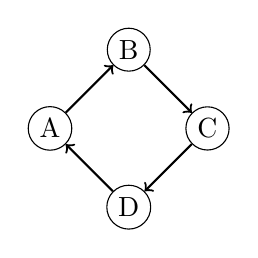
\begin{tikzpicture}[scale=1, every node/.style={circle, draw, fill=white, inner sep=2pt}]
                    \node (a) at (0,0) {A};
                    \node (b) at (1,1) {B};
                    \node (c) at (2,0) {C};
                    \node (d) at (1,-1) {D};
                    \draw[->, thick] (a) -> (b);
                    \draw[->, thick] (b) -> (c);
                    \draw[->, thick] (c) -> (d);
                    \draw[->, thick] (d) -> (a);
                \end{tikzpicture}
                \caption{Subgrafo}
            \end{subfigure}
            \begin{subfigure}{0.3\textwidth}
                \centering
                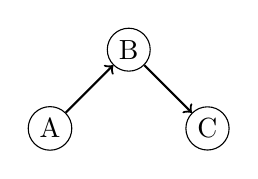
\begin{tikzpicture}[scale=1, every node/.style={circle, draw, fill=white, inner sep=2pt}]
                    \node (a) at (0,0) {A};
                    \node (b) at (1,1) {B};
                    \node (c) at (2,0) {C};
                    \draw[->, thick] (a) -> (b);
                    \draw[->, thick] (b) -> (c);
                \end{tikzpicture}
                \caption{Camino}
            \end{subfigure}
            \begin{subfigure}{0.3\textwidth}
                \centering
                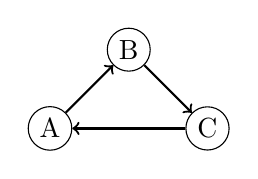
\begin{tikzpicture}[scale=1, every node/.style={circle, draw, fill=white, inner sep=2pt}]
                    \node (a) at (0,0) {A};
                    \node (b) at (1,1) {B};
                    \node (c) at (2,0) {C};
                    \draw[->, thick] (a) -> (b);
                    \draw[->, thick] (b) -> (c);
                    \draw[->, thick] (c) -> (a);
                \end{tikzpicture}
                \caption{Ciclo}
            \end{subfigure}
            \caption{Ejemplos de subgrafo, camino y ciclo en un grafo.}
        \end{figure}

        \subsubsection{Matriz de adyacencia}
            La matriz de adyacencia es una representación matricial que codifica la estructura de un grafo. Dado un grafo $G=(V,E)$ con $N$ vértices, se define una matriz $A \in \mathbb{R}^{N \times N}$, donde cada elemento $a_{ij}$ indica si existe una conexión directa entre el vértice $i$ y el vértice $j$. En un grafo no ponderado:
            \begin{equation}
                a_{ij} =
                \begin{cases}
                    1, & \text{si existe una arista entre } i \text{ y } j,\\
                    0, & \text{en caso contrario.}
                \end{cases}
            \end{equation}
            En grafos ponderados, cada $a_{ij}$ toma el valor del peso asignado a la conexión, lo que permite cuantificar la intensidad o el costo de dicha relación.

    \subsection{Propiedades estructurales}

    Entre las propiedades clásicas que describen la forma en que los vértices se relacionan destacan:
    \begin{itemize}
        \item \textbf{Conectividad}: existe al menos un camino entre cada par de vértices; de lo contrario, la red se fragmenta en componentes conexas.
        \item \textbf{Árbol}: grafo conexo sin ciclos que satisface $|E|=|V|-1$.
        \item \textbf{Diámetro}: longitud del camino más largo entre los caminos más cortos de todos los pares $(u,v)$.
        \item \textbf{Vértice de articulación} e \textbf{istmo}: suprimirlos incrementa el número de componentes, lo que evidencia fragilidad local (Rodrigues, 2013).
        \item \textbf{Número de ciclos independientes}: $\mu = |E|-|V|+p$, donde $p$ es el número de componentes.
    \end{itemize}

    \subsubsection*{Nivel de red}

    \begin{description}

    \item[Índice $\beta$ (conectividad).]
    Mide cuántas aristas existen respecto al número de vértices, es decir, cuántas conexiones “promedio” puede esperar cada vértice. Valores cercanos a $1$ indican una topología arborescente (pocas alternativas de ruta), mientras que valores crecientes reflejan mayor interconexión y, por tanto, más opciones de recorrido.
    \begin{center}
    $\displaystyle \beta \;=\; \frac{|E|}{|V|}$
    \end{center}

    \item[Índice $\alpha$ (redundancia).]
    Cuantifica la proporción de ciclos presentes frente al máximo posible en un grafo planar. Sirve para valorar la resiliencia de la red: cuanto más alto, más caminos alternativos existen ante fallos o congestión. El parámetro $p$ indica el número de componentes conexas (en la práctica, $p=1$ si la red está totalmente conectada).
    \begin{center}
    $\displaystyle \alpha \;=\; \frac{|E| - |V| + p}{\,2|V| - 5\,}$
    \end{center}

    \item[Índice $\gamma$ (densidad planar).]
    Expresa la fracción de aristas observadas respecto del límite superior para un grafo planar simple ($3|V|-6$). Un $\gamma$ cercano a $1$ denota proximidad a la máxima densidad planar, mientras que valores bajos sugieren poca malla y mayor fragilidad estructural.
    \begin{center}
    $\displaystyle \gamma \;=\; \frac{|E|}{\,3|V| - 6\,}$
    \end{center}

    \item[Longitud total.]
    Suma de las longitudes físicas de todas las aristas—por ejemplo, distancia vial o duración promedio del trayecto—que constituye un indicador agregado de la inversión material o de la “extensión” operativa de la red.
    \begin{center}
    $\displaystyle L(G) \;=\; \sum_{(i,j)\in E} \ell_{ij}$
    \end{center}

    \item[Índice de rodeo ($DI$).]
    Compara la distancia efectiva que un viajero recorre sobre la red ($D_S$) con la distancia euclidiana ($D_T$) entre origen y destino. Valores mayores que $1$ revelan desvíos relevantes (trayectorias poco rectas), mientras que valores cercanos a $1$ implican rutas casi directas.
    \begin{center}
    $\displaystyle DI \;=\; \frac{D_S}{D_T}$
    \end{center}

    \item[Brecha espectral ($\Delta$).]
    Diferencia entre el mayor y el segundo mayor autovalor del operador de transición (o del Laplaciano normalizado). Una brecha grande suele asociarse con redes más “cohesivas” y con tiempos de mezcla rápidos para procesos de difusión (p.\,ej., reparto de pasajeros).
    \begin{center}
    $\displaystyle \Delta \;=\; \lambda_{1} - \lambda_{2}$
    \end{center}

    \end{description}

    \subsubsection*{Nivel de vértice}

    \begin{description}

    \item[Grado ($\deg$).]
    Número de aristas incidentes en un vértice. En redes dirigidas se distingue entre grado de entrada ($\deg^{-}$) y grado de salida ($\deg^{+}$); su suma refleja la importancia local del vértice como punto de transferencia.
    \begin{center}
    $\displaystyle \deg(v) \;=\; \deg^{-}(v) + \deg^{+}(v)$
    \end{center}

    \item[Centralidad de cercanía ($C_c$).]
    Mide qué tan “cerca” se encuentra un vértice de todos los demás en términos de distancia sobre la red. Valores elevados (distancias promedio bajas) indican alta accesibilidad global, útil para ubicar terminales o centros de transbordo.
    \begin{center}
    $\displaystyle C_c(v) \;=\; \frac{1}{\sum_{u\in V} d(u,v)}$
    \end{center}

    \item[Centralidad de intermediación ($C_b$).]
    Proporción de rutas geodésicas (más cortas) entre pares de vértices que pasan por $v$. Detecta “puentes” críticos cuyo fallo incrementaría la longitud de los recorridos o desconectaría sectores.
    \begin{center}
    $\displaystyle C_b(v) \;=\; \sum_{s\neq v\neq t}\frac{\sigma_{st}(v)}{\sigma_{st}}$
    \end{center}

    \item[Eccentricidad ($e$).]
    Máxima distancia desde $v$ hacia cualquier otro vértice. Representa el “peor caso” de accesibilidad individual; vértices con baja eccentricidad pueden considerarse estratégicos dentro de la red.
    \begin{center}
    $\displaystyle e(v) \;=\; \max_{u\in V} d(u,v)$
    \end{center}

    \end{description}

    Conjuntamente, estos indicadores permiten diagnosticar fortalezas y debilidades tanto globales como locales, fundamentando decisiones sobre expansión, mantenimiento y robustecimiento de la infraestructura de transporte (Rodrigues, 2013).


    \subsection{Vulnerabilidad y resiliencia}

    Para cuantificar la sensibilidad de la red ante fallos se emplea la \emph{eficiencia global}
    \begin{equation}
        E(G)=\frac{1}{N(N-1)}\sum_{i\neq j}\frac{1}{d_{ij}},
    \end{equation}
    donde $N=|V|$ y $d_{ij}$ denota la longitud del camino más corto entre $i$ y $j$. Si se elimina un conjunto crítico $H$ de vértices (o aristas), la eficiencia resultante es $E(G\setminus H)$ y la \textbf{vulnerabilidad} se define como
    \begin{equation}
        V=\frac{E(G)-E(G\setminus H)}{E(G)}.
    \end{equation}
    Valores altos de $V$ implican que pocos elementos concentran gran parte del flujo: la red es frágil (Rodrigues, 2013).

    \subsection{Algoritmos fundamentales en teoría de grafos}
        Los algoritmos en teoría de grafos permiten resolver problemas como la determinación de caminos más cortos entre vértices. En esta sección se presentan dos algoritmos esenciales para este propósito: Dijkstra y Floyd–Warshall.

        \subsubsection{Algoritmo de Dijkstra}

        El algoritmo de Dijkstra encuentra el camino más corto desde un vértice fuente $s$ hacia todos los demás vértices en un grafo ponderado con pesos no negativos. Se basa en una estrategia voraz que mantiene un conjunto de vértices visitados y actualiza iterativamente las distancias mínimas conocidas.

        \textbf{Entrada:}
        \begin{itemize}
            \item Un grafo dirigido o no dirigido $G = (V, E)$ con pesos no negativos $w: E \to \mathbb{R}^+$.
            \item Un vértice fuente $s \in V$.
        \end{itemize}

        \textbf{Salida:}
        \begin{itemize}
            \item Distancias mínimas $d(v)$ desde $s$ hacia cada $v \in V$.
            \item Árbol de caminos más cortos.
        \end{itemize}

        \textbf{Procedimiento:}
        \begin{enumerate}
            \item Inicializar $d(s) = 0$ y $d(v) = \infty$ para todos $v \neq s$.
            \item Crear un conjunto de vértices visitados $S = \emptyset$.
            \item Mientras $S \neq V$:
            \begin{enumerate}
                \item Seleccionar el vértice $u \notin S$ con la menor distancia $d(u)$.
                \item Agregar $u$ a $S$.
                \item Para cada vecino $v$ de $u$ tal que $(u,v) \in E$:
                \begin{itemize}
                    \item Si $d(u) + w(u,v) < d(v)$, actualizar $d(v) = d(u) + w(u,v)$.
                \end{itemize}
            \end{enumerate}
        \end{enumerate}

        \subsubsection{Algoritmo de Floyd–Warshall}

        El algoritmo de Floyd–Warshall halla los caminos más cortos entre todos los pares de vértices en un grafo ponderado con pesos arbitrarios (incluidos negativos), siempre que no existan \emph{ciclos de peso negativo}. Se basa en programación dinámica y mejora iterativamente una matriz de distancias.

        \textbf{Entrada:}
        \begin{itemize}
            \item Un grafo dirigido $G = (V, E)$ con una matriz de pesos $W$.
        \end{itemize}

        \textbf{Salida:}
        \begin{itemize}
            \item Una matriz $D$ donde $D[i][j]$ representa la distancia más corta entre los vértices $i$ y $j$.
        \end{itemize}

        \textbf{Procedimiento:}
        \begin{enumerate}
            \item Inicializar $D$ como la matriz de adyacencia ponderada $W$: $D[i][j] = w(i,j)$ si existe una arista $(i,j)$, y $\infty$ en caso contrario; además, $D[i][i]=0$ para todo $i$.
            \item Para cada vértice intermedio $k \in V$:
            \begin{enumerate}
                \item Para cada par de vértices $i, j \in V$:
                \begin{itemize}
                    \item Si $D[i][k] + D[k][j] < D[i][j]$, actualizar $D[i][j] = D[i][k] + D[k][j]$.
                \end{itemize}
            \end{enumerate}
        \end{enumerate}
